\documentclass[border=10pt]{standalone}
\usepackage{tikz}
\usetikzlibrary{arrows.meta,decorations.markings,3d}
\usepackage{amsmath}

\begin{document}
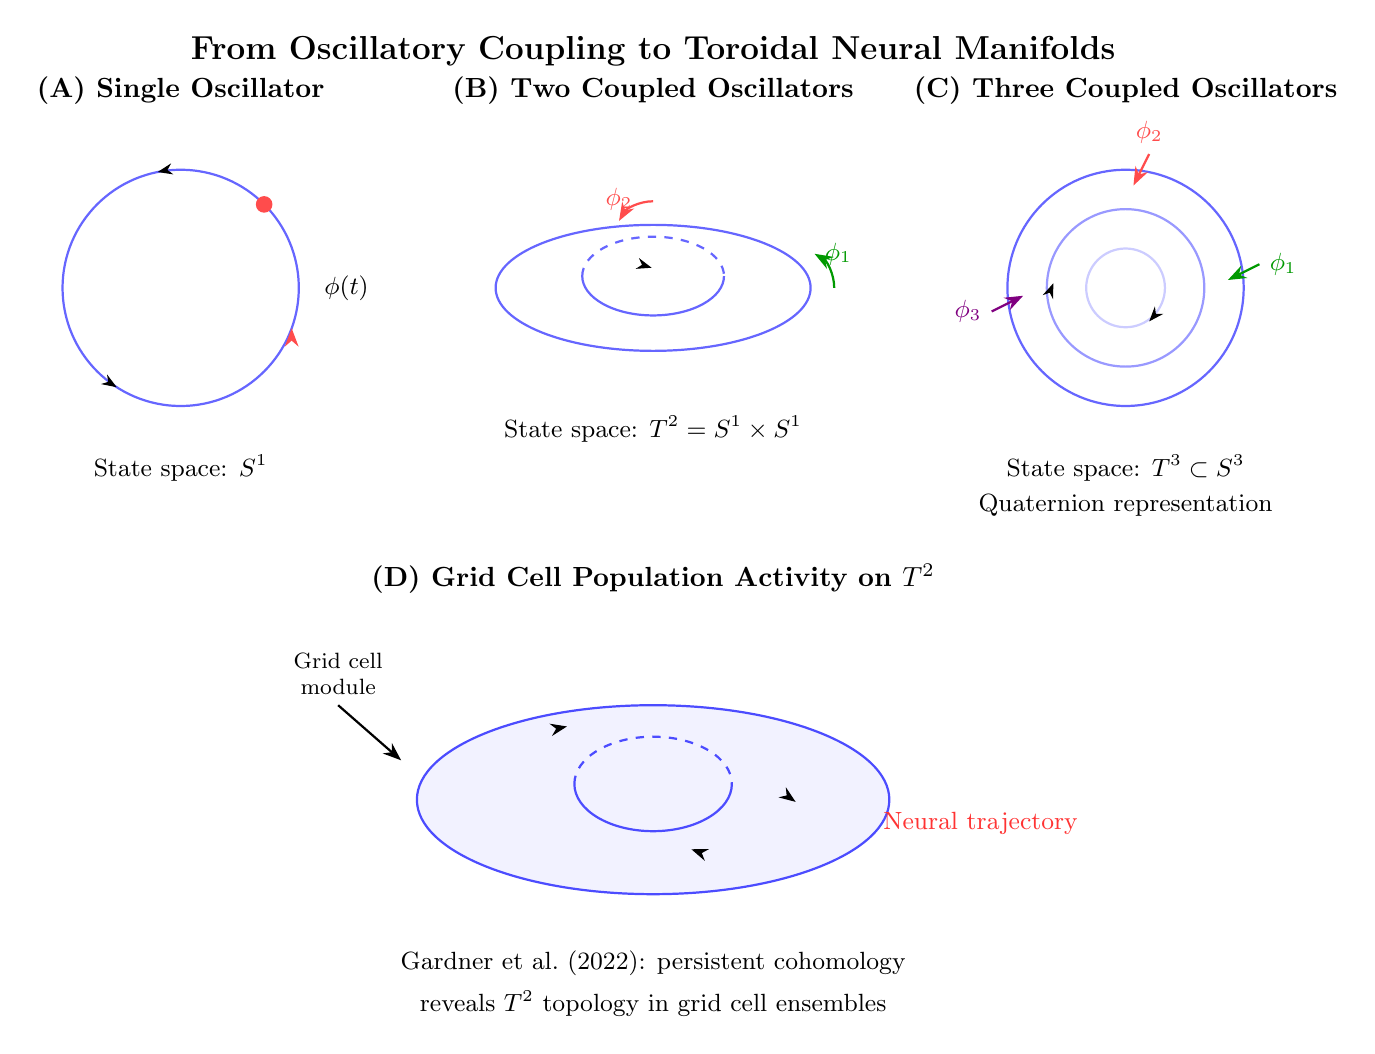
\begin{tikzpicture}[>=Stealth, font=\small]

% --- Panel A: Single oscillator -> circle ---
\begin{scope}[shift={(-6,3)}]
  \node[above, font=\bfseries] at (0,2.2) {(A) Single Oscillator};
  \draw[thick, blue!60] (0,0) circle (1.5);
  \draw[->, thick, red!70, decorate, decoration={markings, mark=at position 0.3 with {\arrow{>}}, mark=at position 0.7 with {\arrow{>}}}] 
    (1.5,0) arc (0:340:1.5);
  \node[right] at (1.7,0) {$\phi(t)$};
  \node[below] at (0,-2) {State space: $S^1$};
  \fill[red!70] (1.06,1.06) circle (3pt);
\end{scope}

% --- Panel B: Two coupled oscillators -> torus ---
\begin{scope}[shift={(0,3)}]
  \node[above, font=\bfseries] at (0,2.2) {(B) Two Coupled Oscillators};
  % Draw torus outline (simplified)
  \draw[thick, blue!60] (0,0) ellipse (2 and 0.8);
  \draw[thick, blue!60] (-0.9,0.15) arc (180:360:0.9 and 0.5);
  \draw[thick, blue!60, dashed] (-0.9,0.15) arc (180:0:0.9 and 0.5);
  % Phase arrows
  \draw[->, thick, green!60!black] (2.3,0) arc (0:60:0.5) node[right] {$\phi_1$};
  \draw[->, thick, red!70] (0,1.1) arc (90:150:0.5) node[above] {$\phi_2$};
  % Trajectory hint
  \draw[thick, orange, dashed, decorate, decoration={markings, mark=at position 0.5 with {\arrow{>}}}] 
    (-1.5,0.3) .. controls (-0.5,0.8) and (0.5,-0.3) .. (1.5,0.2);
  \node[below] at (0,-1.5) {State space: $T^2 = S^1 \times S^1$};
\end{scope}

% --- Panel C: Three coupled -> quaternion S^3 ---
\begin{scope}[shift={(6,3)}]
  \node[above, font=\bfseries] at (0,2.2) {(C) Three Coupled Oscillators};
  % Draw hypersphere projection (simplified as nested circles)
  \draw[thick, blue!60] (0,0) circle (1.5);
  \draw[thick, blue!40] (0,0) circle (1.0);
  \draw[thick, blue!20] (0,0) circle (0.5);
  % Phase arrows
  \draw[->, thick, green!60!black] (1.7,0.3) node[right] {$\phi_1$} -- (1.3,0.1);
  \draw[->, thick, red!70] (0.3,1.7) node[above] {$\phi_2$} -- (0.1,1.3);
  \draw[->, thick, violet] (-1.7,-0.3) node[left] {$\phi_3$} -- (-1.3,-0.1);
  % Trajectory
  \draw[thick, orange, dashed, decorate, decoration={markings, mark=at position 0.3 with {\arrow{>}}, mark=at position 0.7 with {\arrow{>}}}] 
    (0.5,1.4) .. controls (1.2,0.5) and (0.3,-1.0) .. (-1.0,-1.1) .. controls (-1.3,0.2) and (-0.2,1.3) .. (0.5,1.4);
  \node[below] at (0,-2) {State space: $T^3 \subset S^3$};
  \node[below] at (0,-2.5) {Quaternion representation};
\end{scope}

% --- Panel D: Grid cell toroidal manifold ---
\begin{scope}[shift={(0,-3.5)}]
  \node[above, font=\bfseries] at (0,2.5) {(D) Grid Cell Population Activity on $T^2$};
  
  % Draw a better torus
  % Outer ellipse
  \draw[thick, blue!70, fill=blue!5] (0,0) ellipse (3 and 1.2);
  % Inner hole
  \draw[thick, blue!70] (-1.0,0.2) arc (180:360:1.0 and 0.6);
  \draw[thick, blue!70, dashed] (-1.0,0.2) arc (180:0:1.0 and 0.6);
  
  % Trajectory on torus (population activity path)
  \draw[very thick, red!80, decorate, decoration={markings, 
    mark=at position 0.15 with {\arrow{>}}, 
    mark=at position 0.45 with {\arrow{>}},
    mark=at position 0.75 with {\arrow{>}}}] 
    (-2.5,0.3) .. controls (-1.5,1.0) and (-0.3,1.2) .. (0.5,0.8) 
    .. controls (1.3,0.4) and (2.0,-0.2) .. (2.5,-0.5)
    .. controls (2.8,-0.8) and (2.0,-1.0) .. (1.0,-0.8)
    .. controls (0,-0.5) and (-1.0,0.0) .. (-2.0,0.4);
  
  % Labels
  \node[right, red!80] at (2.8,-0.3) {Neural trajectory};
  \node[below] at (0,-1.8) {Gardner et al.\ (2022): persistent cohomology};
  \node[below] at (0,-2.3) {reveals $T^2$ topology in grid cell ensembles};
  
  % Module label
  \draw[<-, thick] (-3.2,0.5) -- (-4.0,1.2) node[above, align=center, font=\footnotesize] {Grid cell\\module};
\end{scope}

% Title
\node[font=\large\bfseries] at (0,6) {From Oscillatory Coupling to Toroidal Neural Manifolds};

\end{tikzpicture}
\end{document}
